\documentclass[11pt]{article}

\usepackage{textcomp}
\usepackage{graphicx}
\usepackage{url}
\usepackage{hyperref}

\usepackage{marvosym}

\usepackage[svgnames]{xcolor}
%% \definecolor{lightgrey}{rgb}{0.7,0.7,0.7}
%% \definecolor{grey}{rgb}{0.5,0.5,0.5}


\setlength{\oddsidemargin}{20pt}
\setlength{\topmargin}{-50pt}
\setlength{\textwidth}{6in}
\setlength{\textheight}{670pt}

\setlength{\parindent}{0pt}
\setlength{\parskip}{10pt}

\pagestyle{empty}

\renewcommand{\baselinestretch}{1.1}

\newcommand{\etal}{\textit{et al.}}

\begin{document}

\sffamily 


\raisebox{-4pt}{
%% \includegraphics[width=0.4\textwidth]{uvm-towerlogoK.png}
%% \includegraphics[width=0.4\textwidth]{uvm-towerlogo2C.jpg}

\includegraphics[width=0.2\textwidth]{roboctopus.png}
%% \includegraphics[height=68pt]{psd_1.jpg}
}
% \textcolor{DarkSlateBlue}{
{ \small
\begin{tabular}[b]{l}
Prof.\ Peter Sheridan Dodds\\
Director of the Vermont Complex Systems Center\\
Co-Director, Computational Story Lab\\
%% \Letter\
%% Department of Mathematics and Statistics\\
%% University of Vermont\\
210 Colchester Avenue, Burlington, VT, 05401, USA\\
%% \Lightning
%% \Email\
pdodds@uvm.edu
$\bullet$
http://www.uvm.edu/{$\sim$}pdodds
% \Mobilefone
% +1-917-533-8135 % (cell)
% $\bullet$
% \Telefon 
% +1-802-656-3089 % (home)
\end{tabular}
}
% \raisebox{-16pt}{
% \includegraphics[height=68pt]{psd_1.jpg}
% }


\bigskip
\bigskip

To the Editors,

We are very pleased to submit our manuscript for consideration at the Journal of Computational Science:\\
\textbf{``Connecting every bit of knowledge:
The structure of Wikipedia\textquotesingle s First Link Network''.}

Our major contributions and findings are as follows:

\textbf{1.}
We connect all 4.7 million Wikipedia articles in a directed network via the first link.
The network reflects how the many inventions, places, figures, objects, and events are related and organized.

\textbf{2.}
We develop a novel algorithm to map the structure of a directed network as a flow. Our measures quantify: \\
\mbox{}\ \textbf{a.}
where references accumulate\\
\mbox{}\ \textbf{b.}
groups of path-connected nodes\\
\mbox{}\ \textbf{c.}
the influence each node exerts in shaping the network.

\textbf{3.}
We identify a gravitation of references on Wikipedia from  specific to general, which culminates disproportionately around only a few fundamental notions. 


Our findings form the basis for a new network-based topic search engine with applications in natural language processing and cognitive psychology.

We look forward to hearing your decision.

Yours sincerely and on behalf of the manuscript's authors,

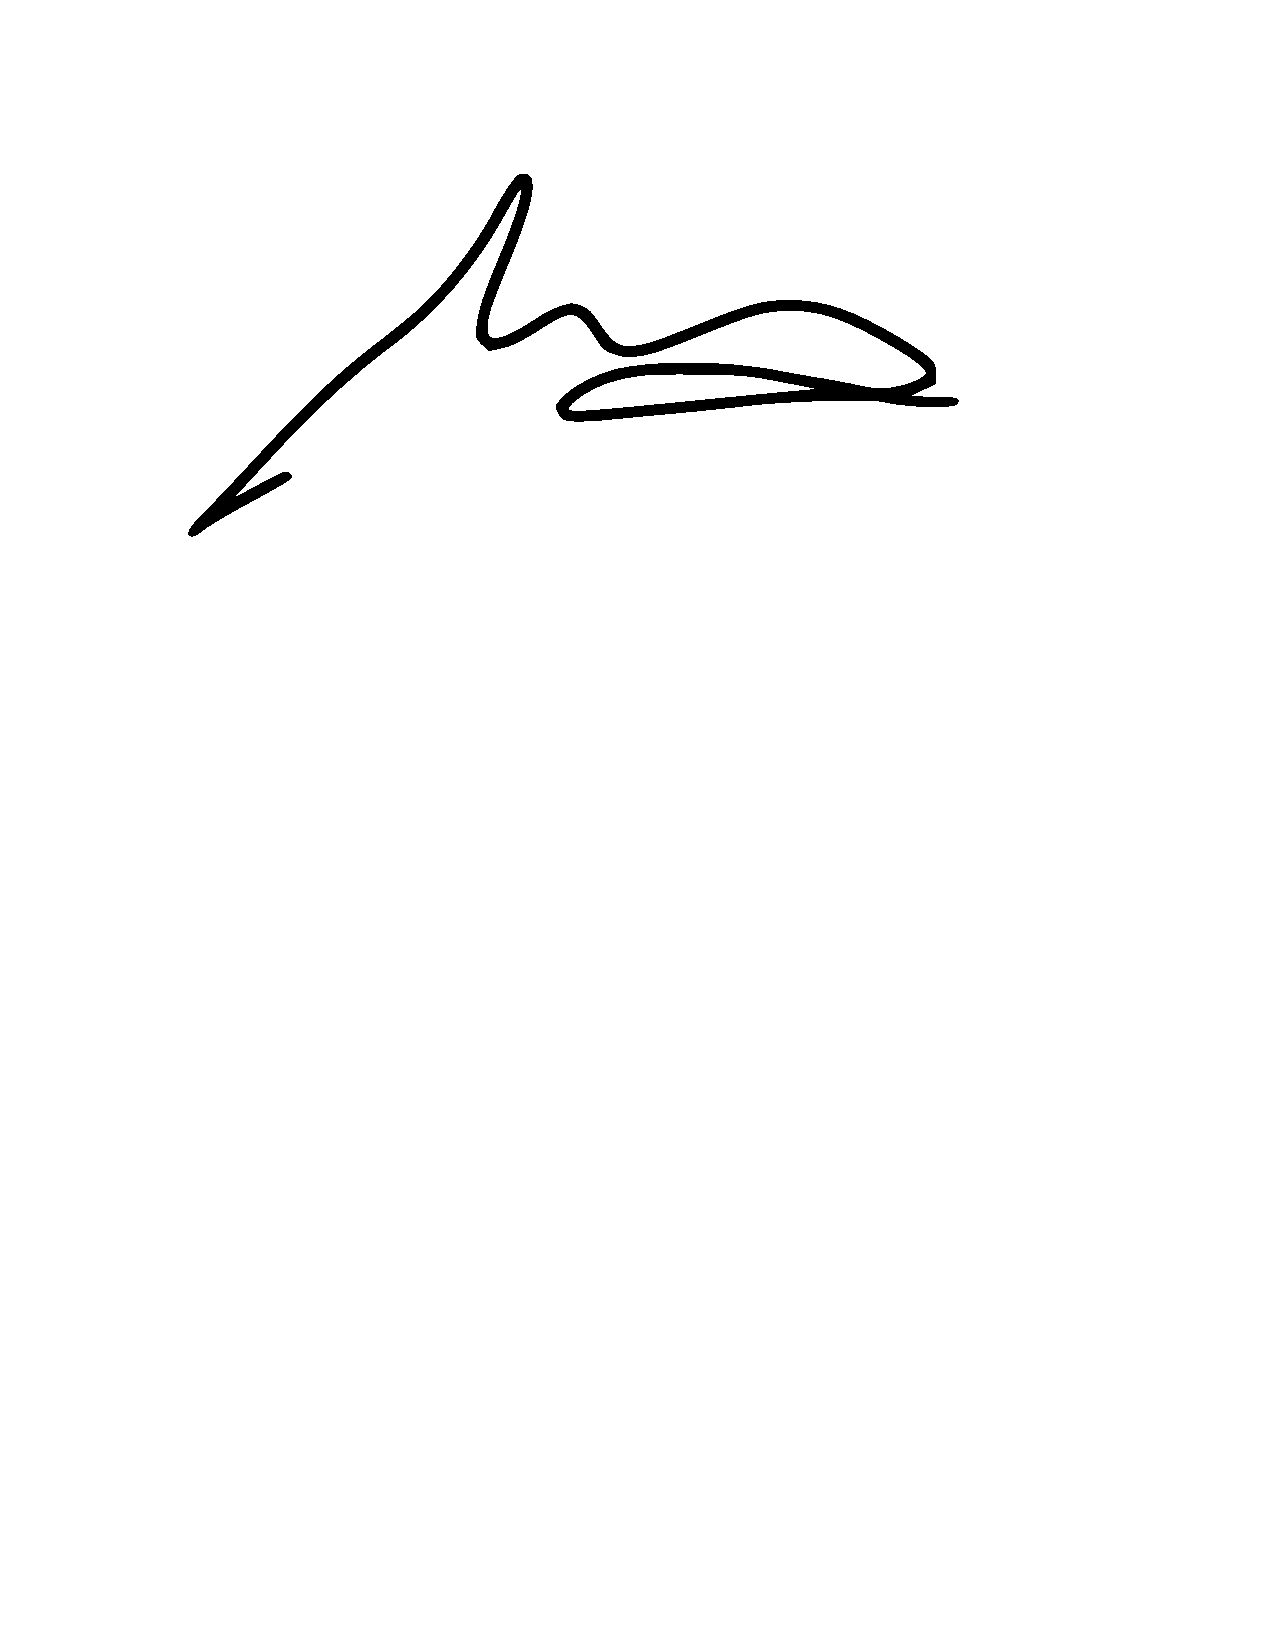
\includegraphics[width=0.2\textwidth]{signature}\\
Mark Ibrahim

%% {\small
%% Professor\\
%% Director of the Vermont Complex Systems Center\\
%% Co-Director, Computational Story Lab\\
%% Vermont Advanced Computing Core\\
%% Department of Mathematics and Statistics\\
%% University of Vermont\\
%% 

% $\bullet$ 
% Department of Mathematics and Statistics\\
% $\bullet$ 
% Vermont Advanced Computing Center\\
% $\bullet$ 
% Complex Systems Center\\
% University of Vermont\\
% pdodds@uvm.edu
% $\bullet$
% http://www.uvm.edu/{$\sim$}pdodds

%% \textbf{Suggested reviewers and their relevant expertise:}


\end{document}
